% Auto-generated from experiment results.
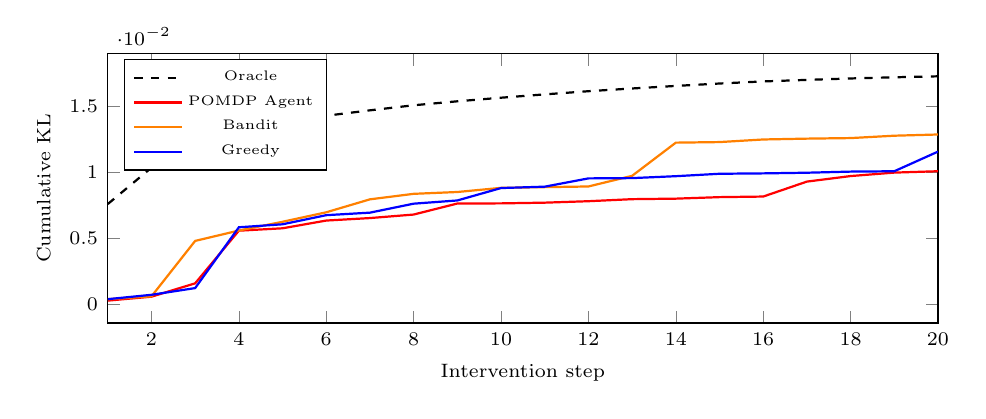
\begin{tikzpicture}
\begin{axis}[
    width=\columnwidth,
    height=5cm,
    xlabel={Intervention step},
    ylabel={Cumulative KL},
    x label style={font=\scriptsize},
    y label style={font=\scriptsize},
    tick label style={font=\scriptsize},
    legend style={
        font=\tiny,
        at={(0.02,0.98)},
        anchor=north west
    },
    xmin=1, xmax=20,
]

\addplot[black, dashed, thick] coordinates { (1,0.007569) (2,0.010324) (3,0.012028) (4,0.013152) (5,0.013773) (6,0.014261) (7,0.014671) (8,0.015055) (9,0.015355) (10,0.015627) (11,0.015880) (12,0.016120) (13,0.016327) (14,0.016520) (15,0.016703) (16,0.016861) (17,0.016978) (18,0.017086) (19,0.017175) (20,0.017249) };
\addplot[red, thick] coordinates { (1,0.000251) (2,0.000549) (3,0.001560) (4,0.005550) (5,0.005732) (6,0.006318) (7,0.006507) (8,0.006773) (9,0.007609) (10,0.007620) (11,0.007674) (12,0.007784) (13,0.007939) (14,0.007978) (15,0.008093) (16,0.008137) (17,0.009270) (18,0.009690) (19,0.009952) (20,0.010056) };
\addplot[orange, thick] coordinates { (1,0.000361) (2,0.000573) (3,0.004776) (4,0.005562) (5,0.006226) (6,0.006944) (7,0.007926) (8,0.008343) (9,0.008482) (10,0.008796) (11,0.008850) (12,0.008900) (13,0.009708) (14,0.012222) (15,0.012265) (16,0.012462) (17,0.012526) (18,0.012568) (19,0.012748) (20,0.012840) };
\addplot[blue, thick] coordinates { (1,0.000361) (2,0.000692) (3,0.001201) (4,0.005808) (5,0.006035) (6,0.006726) (7,0.006917) (8,0.007597) (9,0.007841) (10,0.008781) (11,0.008886) (12,0.009513) (13,0.009535) (14,0.009680) (15,0.009864) (16,0.009893) (17,0.009943) (18,0.010027) (19,0.010054) (20,0.011541) };

\legend{Oracle, POMDP Agent, Bandit, Greedy}

\end{axis}
\end{tikzpicture}
